This section provides a detailed description of the data utilized for my empirical analysis. Furthermore, this section demonstrates a key feature of my research design.


% Institutional Background
\subsection{Background of Residential Rates of Sacramento Municipal Utility District}
\label{C1-Sub-section:Background-of-Residential-Rates-of-SMUD}
Sacramento Municipal Utility District (SMUD), which is the nation's sixth-largest community-owned electric utility, provides electricity to most of Sacramento County and small portions of adjoining Placer and Yolo Counties.\footnote{According to the company information presented on \href{https://www.smud.org/en/Corporate/About-us/Company-Information}{SMUD's website}, the size of this utility's service area is about 900 square miles.}

\afterpage{
    \begin{figure}[t!]
        \centering
        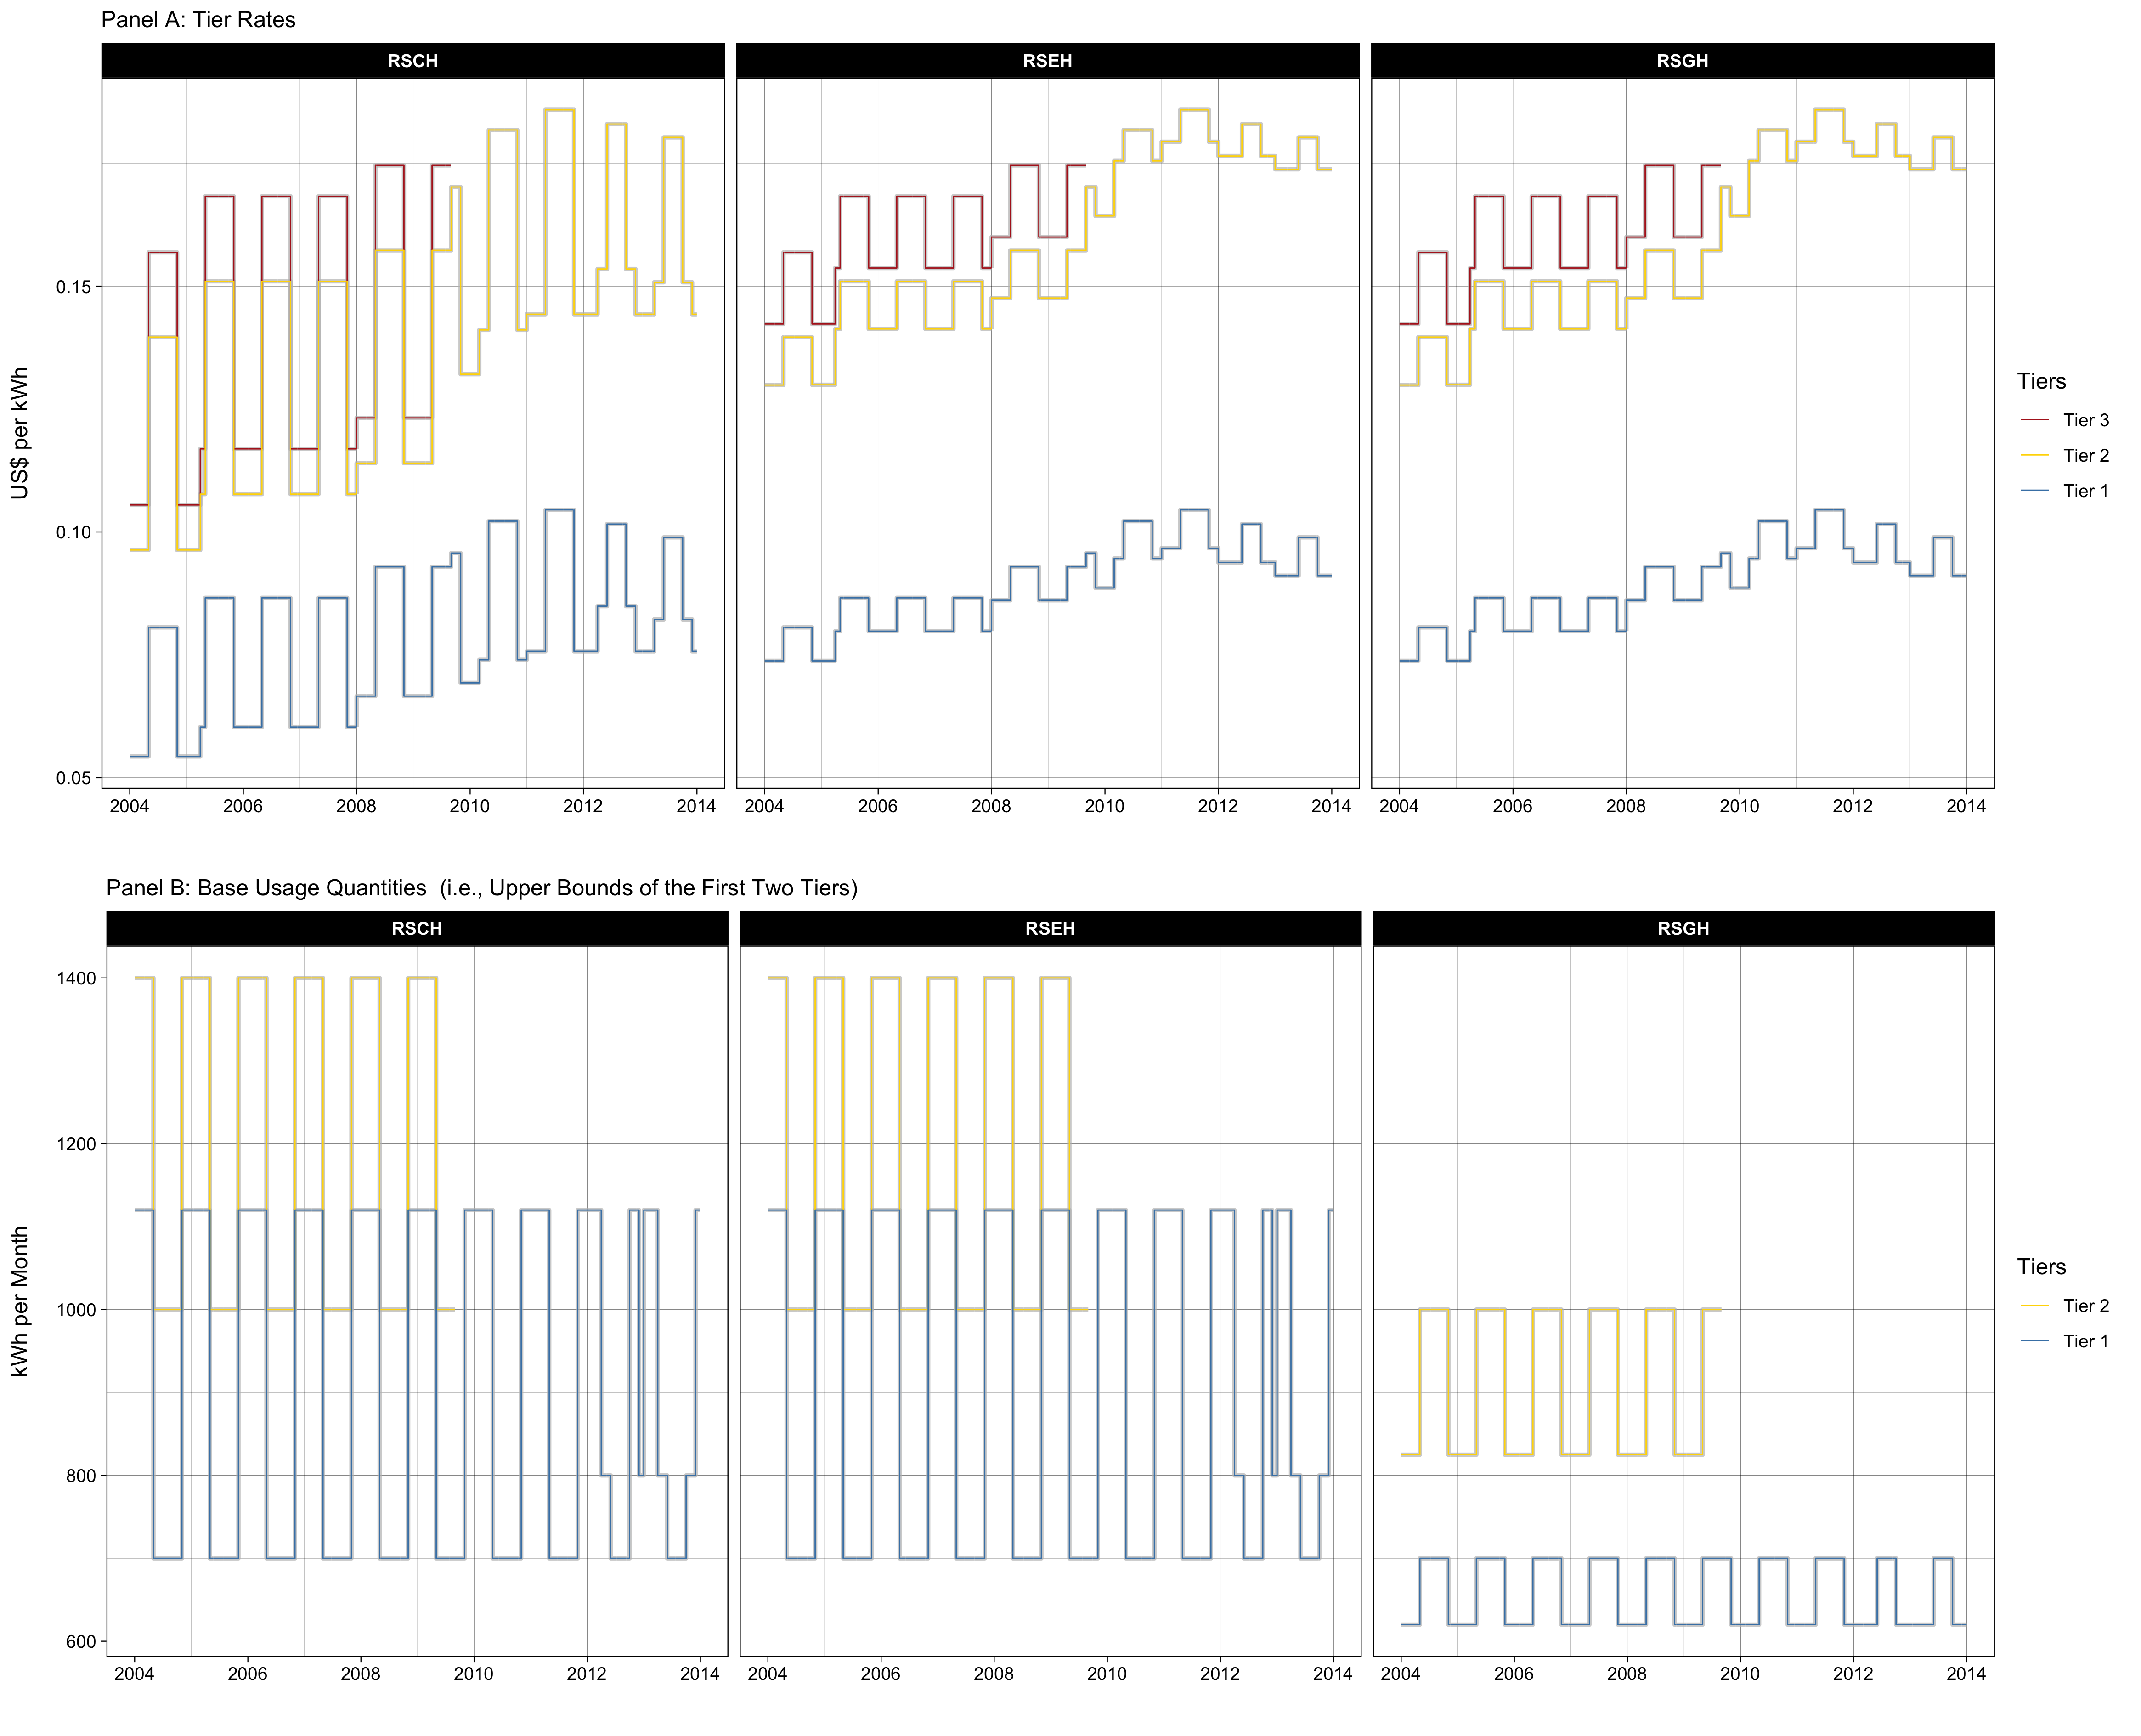
\includegraphics[scale = 0.097]{02_Chapter-1/00A_Figures/Figure_SMUD-Residential-Rates_Variable-Charges-and-Base-Usage-Quantities.png}
        \caption{Tier Rates and Base Usage Quantities of SMUD Residential Rates}
        \caption*{
            {\small
            \textit{Note}: 
            The figure illustrates how SMUD changed tier rates and base usage quantities of the three major residential rate plans (i.e., RSCH, RSEH, and RSGH) over time. Both tier rates and base usage quantities show significant seasonality. The two rate plans for electric-heating households (i.e., RSCH and RSEH) had the same base usage quantities. There have been only two tiers since September 2009.
        }}
        \label{Figure:SMUD-Residential-Rates_Variable-Charge-and-Base-Usage}
    \end{figure}
}
Before the default residential rate switched to the Time-Of-Day (TOD) rate, most SMUD residential customers chose residential rates having an increasing nonlinear block-tier structure.\footnote{In my sample, only 5\% of residential customers adopted the TOD rate, although SMUD already offered it.} The three most popular rates for SMUD residential customers were Standard General Service (RSGH), Standard Closed Electric-Heated Service (RSCH), and Standard Open Electric-Heated Service (RSEH).\footnote{Specifically, more than 75\% of SMUD residential customers in my dataset chose the RSGH rate, whereas 2\% and 20\% of households in my dataset adopted the RSCH and RSEH rates, respectively.} For those residential rates, the marginal price of the energy charge was a step function of monthly consumption relative to a base usage quantity per month, which varies seasonally. Figure \ref{Figure:SMUD-Residential-Rates_Variable-Charge-and-Base-Usage} illustrates variations in price and base usage quantity over time. Two points are noteworthy from this figure: first, both tier rates and base usage quantities of the energy charges showed substantial seasonality; second, the structure of the residential rates changed from three-tier to two-tier since September 2009.

In addition to the variable charge (i.e., the energy charge), households choosing one of the three rates should pay a per-month fixed charge, called the System Infrastructure Fixed Charge. As shown in Figure \ref{Figure:SMUD-Residential-Rates_Fixed-Charge}, the unit price of the fixed charge significantly increased between 2009 and 2014. 




% Data and Summary Statistics
\subsection{Data and Summary Statistics}
\label{C1-Sub-section:Data-and-Summary-Statistics}
From SMUD, I obtain household-level monthly billing history of residential consumers in the Sacramento area from 2004 to 2013. For each monthly record, account ID, premise ID, rate code, billing start and end dates, monthly consumption with its breakdown into each tier, monthly fixed charge, monthly variable charge only for kWh usage, total monthly bill, and an indicator related to solar adoption are included in the data. Of note, in my empirical analysis, I assume that a pair of account and premise IDs corresponds to an individual household. And because the monthly billing data contain no price and base usage quantity information, I append historical price schedules and base usage quantities presented by SMUD. Unfortunately, my monthly billing data also lack any socioeconomic and demographic information. 

First, I focus on households that consistently used one of the three major residential rates (i.e., RSGH, RSCH, and RSEH) in their billing history. Second, I only utilize billing records before 2010, from which SMUD got down to install smart meters. Third, I focus on households whose number of billing periods is greater than or equal to 24. Fourth, I focus on SMUD residential customers with reliable billing records only.\footnote{To be specific, I exclude, from the sample used for my empirical analysis, households that have billing records being applied to any of the following conditions: 1) observations whose length of the billing period is either less than 27 or greater than 34; 2) observations with negative values for either quantities or charges; 3) observations having overlapping billing periods within a pair of account and premise IDs; and 4) observations whose number of days from the previous billing period is greater than 14.} Fifth, my sample only includes households that crossed the lower threshold at least once in their billing history.\footnote{In other words, I drop always-light- and always-heavy-users from my sample. } The procedure results in 16,322,353 billing records for 365,975 households. Table \ref{Table:Summary-Statistics} provides summary statistics for my sample. Furthermore, Figure \ref{Figure:Household-Average-Daily-Electricity-Consumption-by-Month-of-Year} shows, for each rate code, households' average daily electricity consumption by month of the year. 

To take account of the impact of weather conditions, especially outdoor temperatures, on household electricity consumption, I utilize the Local Climatological Data (LCD) for the Sacramento International Airport, published by the National Oceanic and Atmospheric Administration (NOAA). Using daily heating degree days (HDDs) and daily cooling degree days (CDDs) in the LCD between 2004 and 2009, I calculate each monthly billing period's accumulated HDDs and CDDs, which are used to compute the average daily HDDs and CDDs. 




% Research Design
\subsection{Research Design}
\label{C1-Sub-Section:Research-Design}

\subsubsection{Monthly Bill as the Only Source of Electric Usage Information for Households}
\label{C1-Sub-Sub-section:Monthly-Bill-as-the-Only-Source-of-Electric-Usage-Information-for-Households}
Before 2009, there was no feasible way for SMUD residential customers to access real-time information related to their electricity use. SMUD initiated installations of smart meters, allowing its residential and business customers to view their electricity usage online when they want, in late 2009. The electric service completed it in the first quarter of 2012. Also, the three types of bill alert SMUD are offering were introduced in 2017.\footnote{SMUD provides its customers with three types of bill alerts, via text or e-mail, as a billing service: 1) Mid-Bill Alerts send an alert on the 16th day of a customer's billing period and advise what his usage has been and what the cost is as of that day, 2) High Bill Alters compare a customer's current billing cycle to the same billing cycle in the previous year and alerts the customer if their current usage is running higher than before, and 3) Bill Threshold allows a customer to know when his bill has reached a certain amount set in advance by himself.} Therefore, for households using SMUD-delivering electricity, the only practical source of information about their electricity consumption had been their monthly bill statements, which send out (either e-mail or U.S. mail) after 3 or 4 business days from the last day of each billing cycle. 

The issue of households' welfare losses due to their response to discontinuous changes in the lagged marginal price suggests the importance of providing seemly price information in an appropriate manner. Many studies about various time-varying electricity pricing show that households changed their consumption behavior in response to the information about consumption and prices \citep{Dynamic-Pricing-of-Electricity-in-the-Mid-Atlantic-Region_Econometric-Results-from-the-Baltimore-Gas-and-Electric-Company-Experiment_Faruqui-et-al_2011, Knowledge-is-Less-Power_Jessoe-and-Rapson_2014, The-Effect-of-Information-on-TOU-Electricity-Use:An-Irish-Residential-Study_Pon_2017, Information-vs-Automation-and-Implications-for-Dynamic-Pricing_Bollinger-and-Hartmann_2020}. My empirical finding demonstrates that even under IBP, such information, though lagged, still plays a role in household electricity consumption. In this respect, providing household-specific as well as current price information for residential consumers, via text messages or app notifications regularly, could encourage them to respond to \textit{true} price signals rather than lagged ones, which in turn avoid the negative impact on household welfare. Based on the dissipating effect of intermittently salient information discussed in \cite{Dynamic-Salience-with-Intermittent-Billing_Gilbert-and-Zivin_2014}, a high frequency of informing the latest tailored price information might maximize households' behavior change in electricity consumption. In addition, because sending such information-bearing notifications is available at a very low cost these days, this type of information provision would be a practical policy instrument for utilities, especially in developing countries where the transition toward dynamic electricity pricing is difficult due to substantial investments in installing smart metering systems. 


\subsubsection{Regression Discontinuity Design}
\label{C1-Sub-Sub-Section:Regression-Discontinuity-Design}
In this paper, I employ a Regression Discontinuity (RD) design to examine how households' electricity consumption responds to the marginal price informed via monthly energy statements under Increasing-Block Pricing (IBP). In previous studies, a common challenge in measuring consumption responses to price changes has been discussed repeatedly: constructing a well-defined control group is difficult due to that consumers typically experience the same price variation. However, the setting I exploit in this paper enables me to address the identification challenge.  

The RD design I implement in this paper relies on three points. First, the marginal price is a step function of consumption level in the increasing block-tier rate plans chosen by SMUD residential customers. That is, under IBP, the price a household pays for the marginal electricity consumption increases discontinuously at some pre-determined aggregate consumption in a billing cycle. Second, as discussed in Section \ref{C1-Sub-Sub-section:Monthly-Bill-as-the-Only-Source-of-Electric-Usage-Information-for-Households}, before 2009, SMUD residential customers had practically no way to know the marginal price in a billing cycle within the very cycle. They were informed of the price they paid for the marginal electricity consumption in a billing cycle only through their electricity bills delivered in the following cycle. Third, it is not generally feasible for households to consume only a pre-targeted amount of electricity within a billing cycle. In general, households have limited capability to control their electricity consumption due to the minimal essential demand (e.g., usage for refrigerators and lighting). In addition, because household electricity consumption heavily depends on outdoor temperature variation, managing one's own electricity usage not to exceed the target amount of electricity consumption could incur too high information cost, which might result in rational inattention \citep{Rational-Inattention-and-Energy-Efficiency_Sallee_(2014)}, even if households are available to adjust their consumption behavior with complete flexibility. 

\afterpage{
    \begin{figure}[t!]
        \centering
        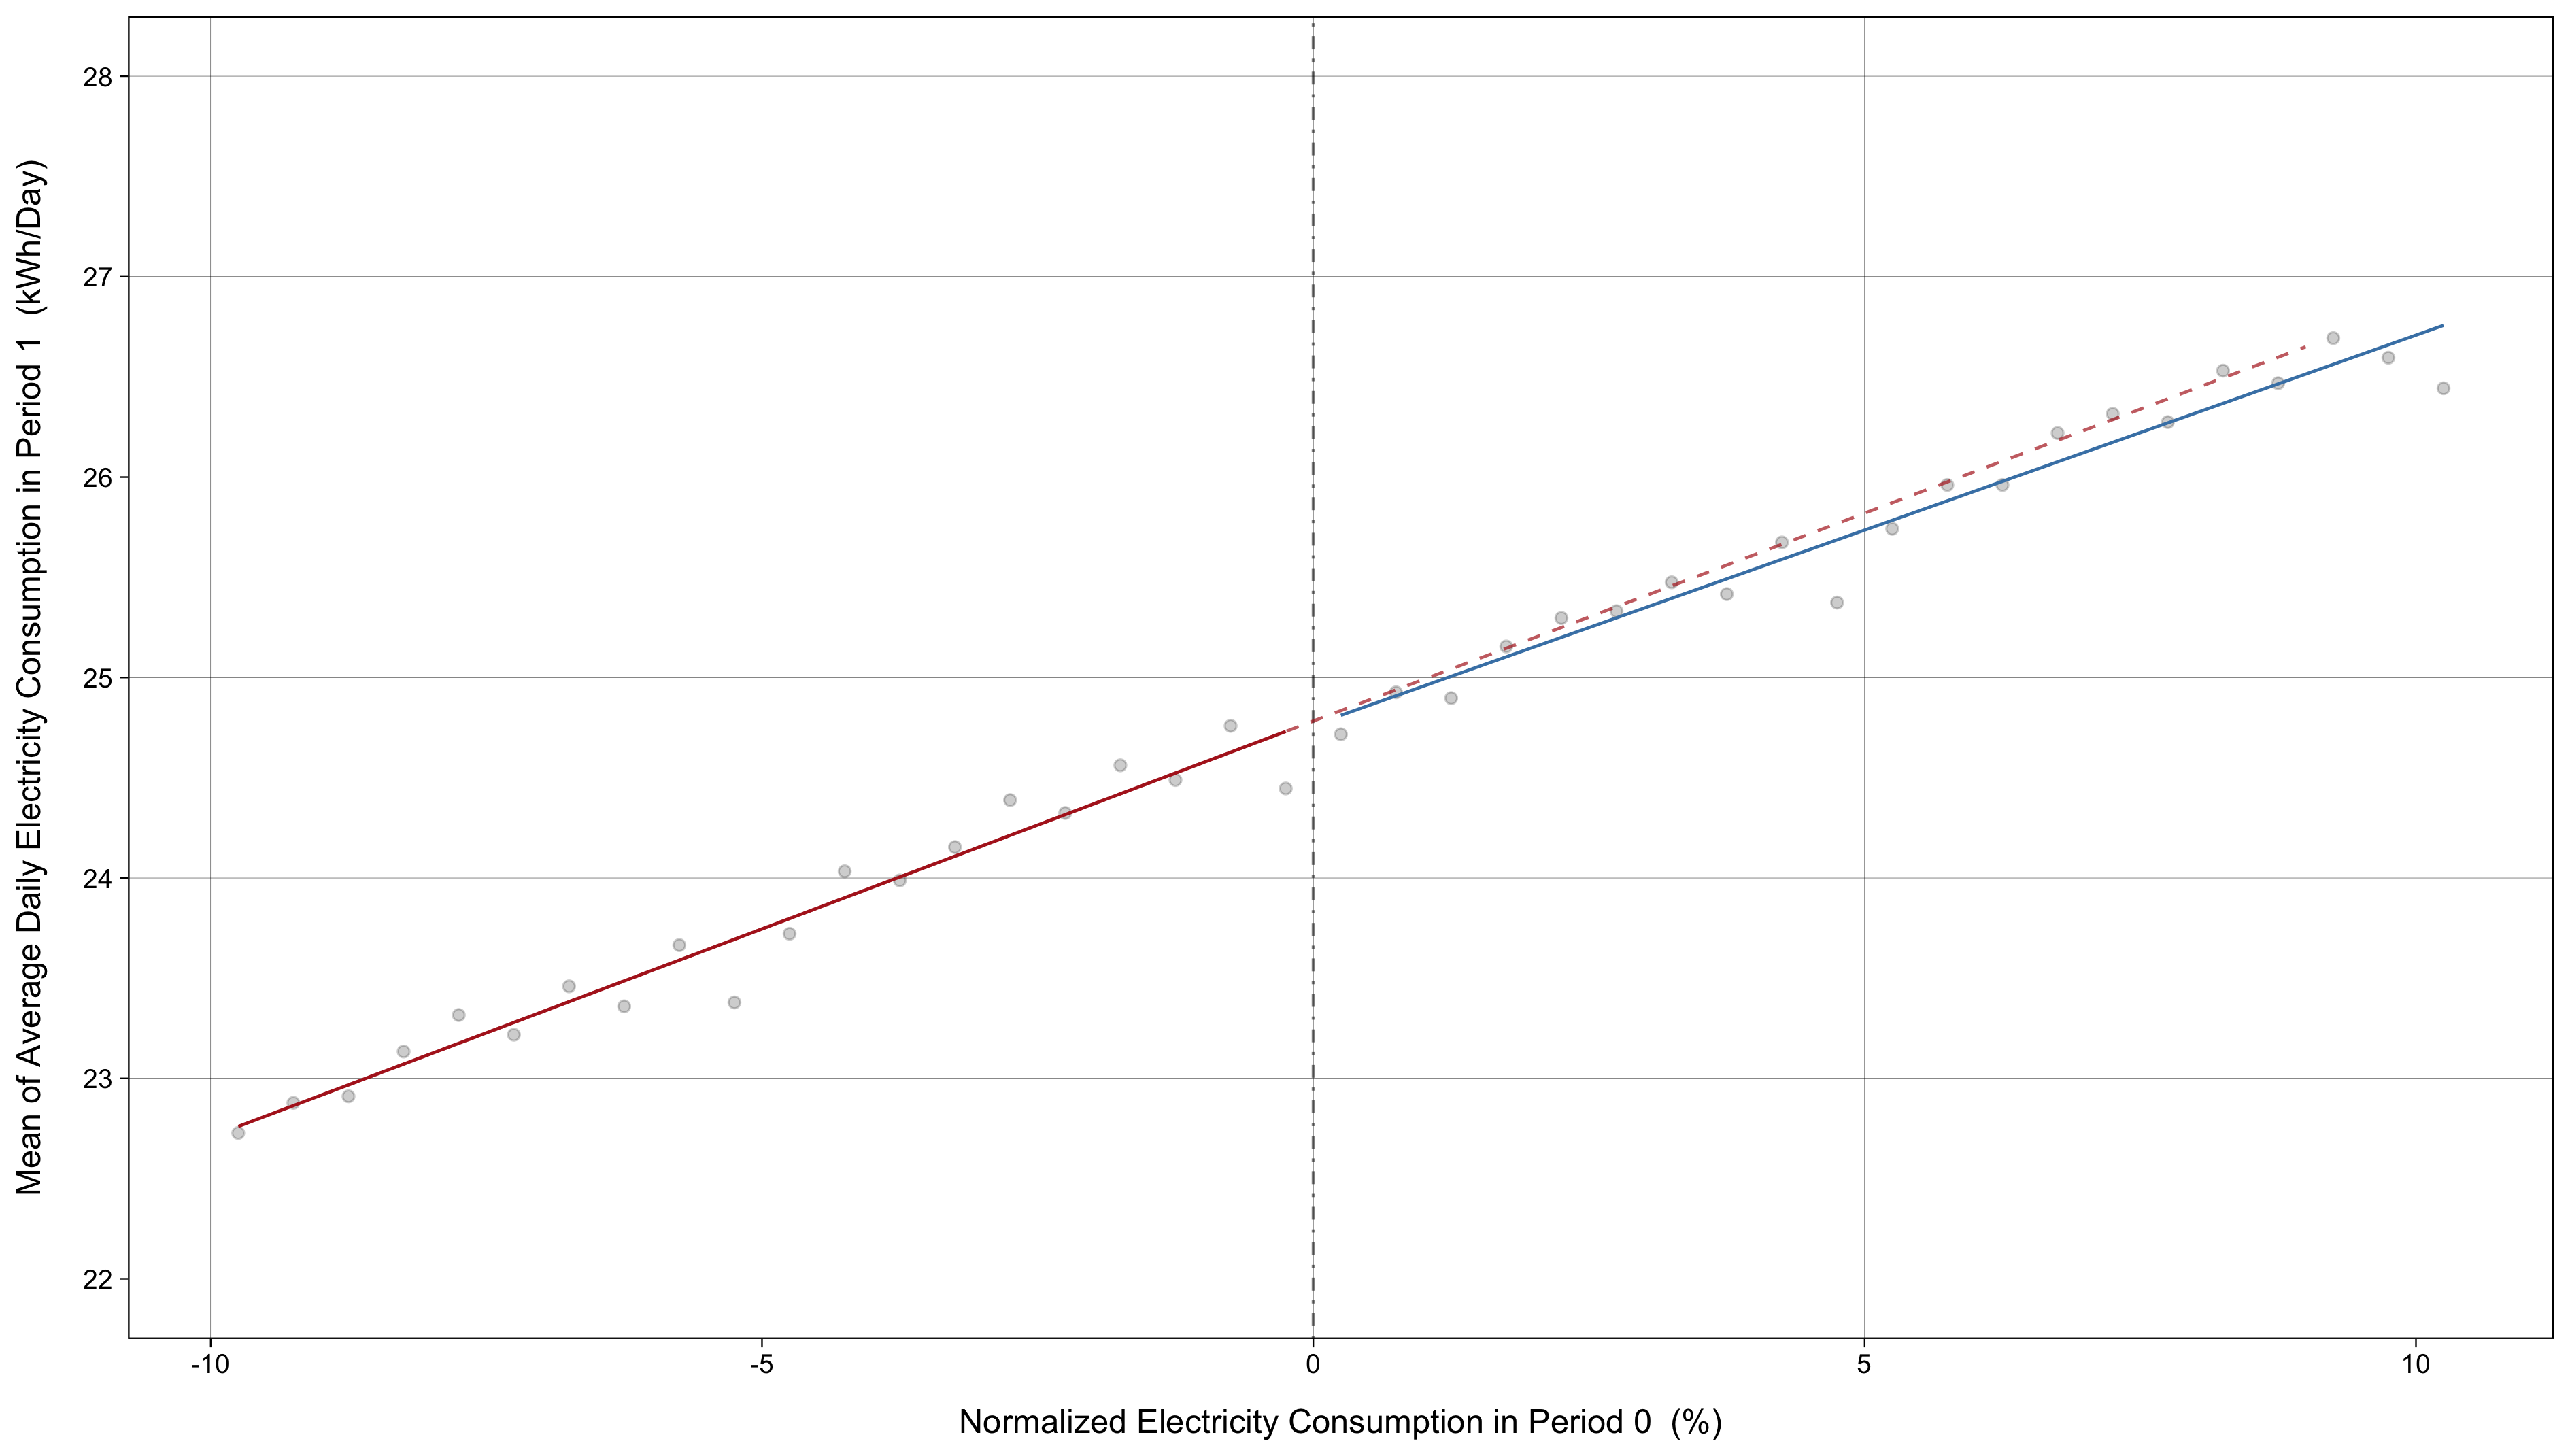
\includegraphics[scale = 0.115]{02_Chapter-1/00A_Figures/Figure_Average-Daily-Electricity-Consumption-in-Period-1-over-NC0.png}
        \caption{Mean of Average Daily Electricity Consumption in Period 1 over $\overline{NC}_{0}$}
        \caption*{
            {\small
            \textit{Note}: 
            This figure's scatter points correspond to the average daily electricity consumption in Period 1, computed by bins with a bandwidth of 1\% of $\overline{NC}_{0}$. The solid line on each side of the vertical dot-dash line is a parametric fit obtained from the regression of the average daily electricity consumption on $\overline{NC}_{0}$. The dashed red line is an extension of the solid red line. The gap between the dashed red and solid blue lines seems to indicate a non-negligible treatment effect. 
        }}
        \label{Figure:Average-Daily-Electricity-Consumption-in-Period-1-over-NC0}
    \end{figure}
}
Regarding the first point, the discontinuities under the nonlinear electricity schedules allow utilizing a RD design. In my RD design, the running variable is the level of electricity consumption in a household during a billing period (denoted as Period 0), whereas the outcome variable corresponds to the household's average daily electricity consumption during the subsequent billing period (denoted as Period 1). So, in this quasi-experimental setting, I compare SMUD residential customers just above and below the thresholds of the tier rates, called base usage quantities. Under IBP, surpassing a threshold leads to an increase in the marginal price households pay for electricity consumption mechanically. Here, the discontinuous increase in the marginal price, which accompanies \textit{no discontinuous change in the average price}, applies only to Period 0, not to Period 1.\footnote{The average price smoothly grows around the cutoff point.} Moreover, information about whether households were subject to a higher marginal price in a billing period is delivered early in the subsequent billing period through their monthly electricity bills. Therefore, any changes with respect to the electricity consumption of households just above the threshold (i.e., households in the treatment group) in Period 1, compared to households just below the threshold (i.e., households in the control group), can be understood as their short-term behavioral responses stemming from the sharp jump in the marginal price in Period 0. Figure \ref{Figure:Average-Daily-Electricity-Consumption-in-Period-1-over-NC0}, showing how the mean of households' average daily electricity consumption in Period 1 evolves around the lower base usage quantity, seems to indicate the existence of such behavioral responses. 

The last two points demonstrate that the fundamental identifying assumption of the RD design is reasonable. The fundamental identifying assumption is that SMUD residential customers just below a base usage quantity are expected to be very similar to those just above it, along with observed and unobserved characteristics. In other words, a group of households in the small neighborhood of the threshold is not different from one obtained from a randomized experiment. In my setting for empirical analysis, SMUD residential customers were unable to be aware of how far away they were from a given cutoff point in real time. Furthermore, as discussed above, it is not convincing that they can perfectly control their electricity consumption during a billing cycle to use exactly a target amount of electricity by the end of the last day of the billing cycle. Hence, it is highly unlikely that the customers precisely adjusted their consumption behavior so as to avoid surpassing the cutoff point, which in turn prevented them from leading to a higher marginal price. That is, it seems plausible that households were not able to sort themselves around the threshold strategically. Therefore, any discontinuity gap in the outcome variable can be attributed to the discontinuous increase in the marginal price at the threshold in Period 0. 


\subsubsection{The Validity of the Regression Discontinuity Design}
\label{C1-Sub-Sub-Section:The-Validity-of-the-Regression-Discontinuity-Design}
\afterpage{
    \begin{figure}[t!]
        \centering
        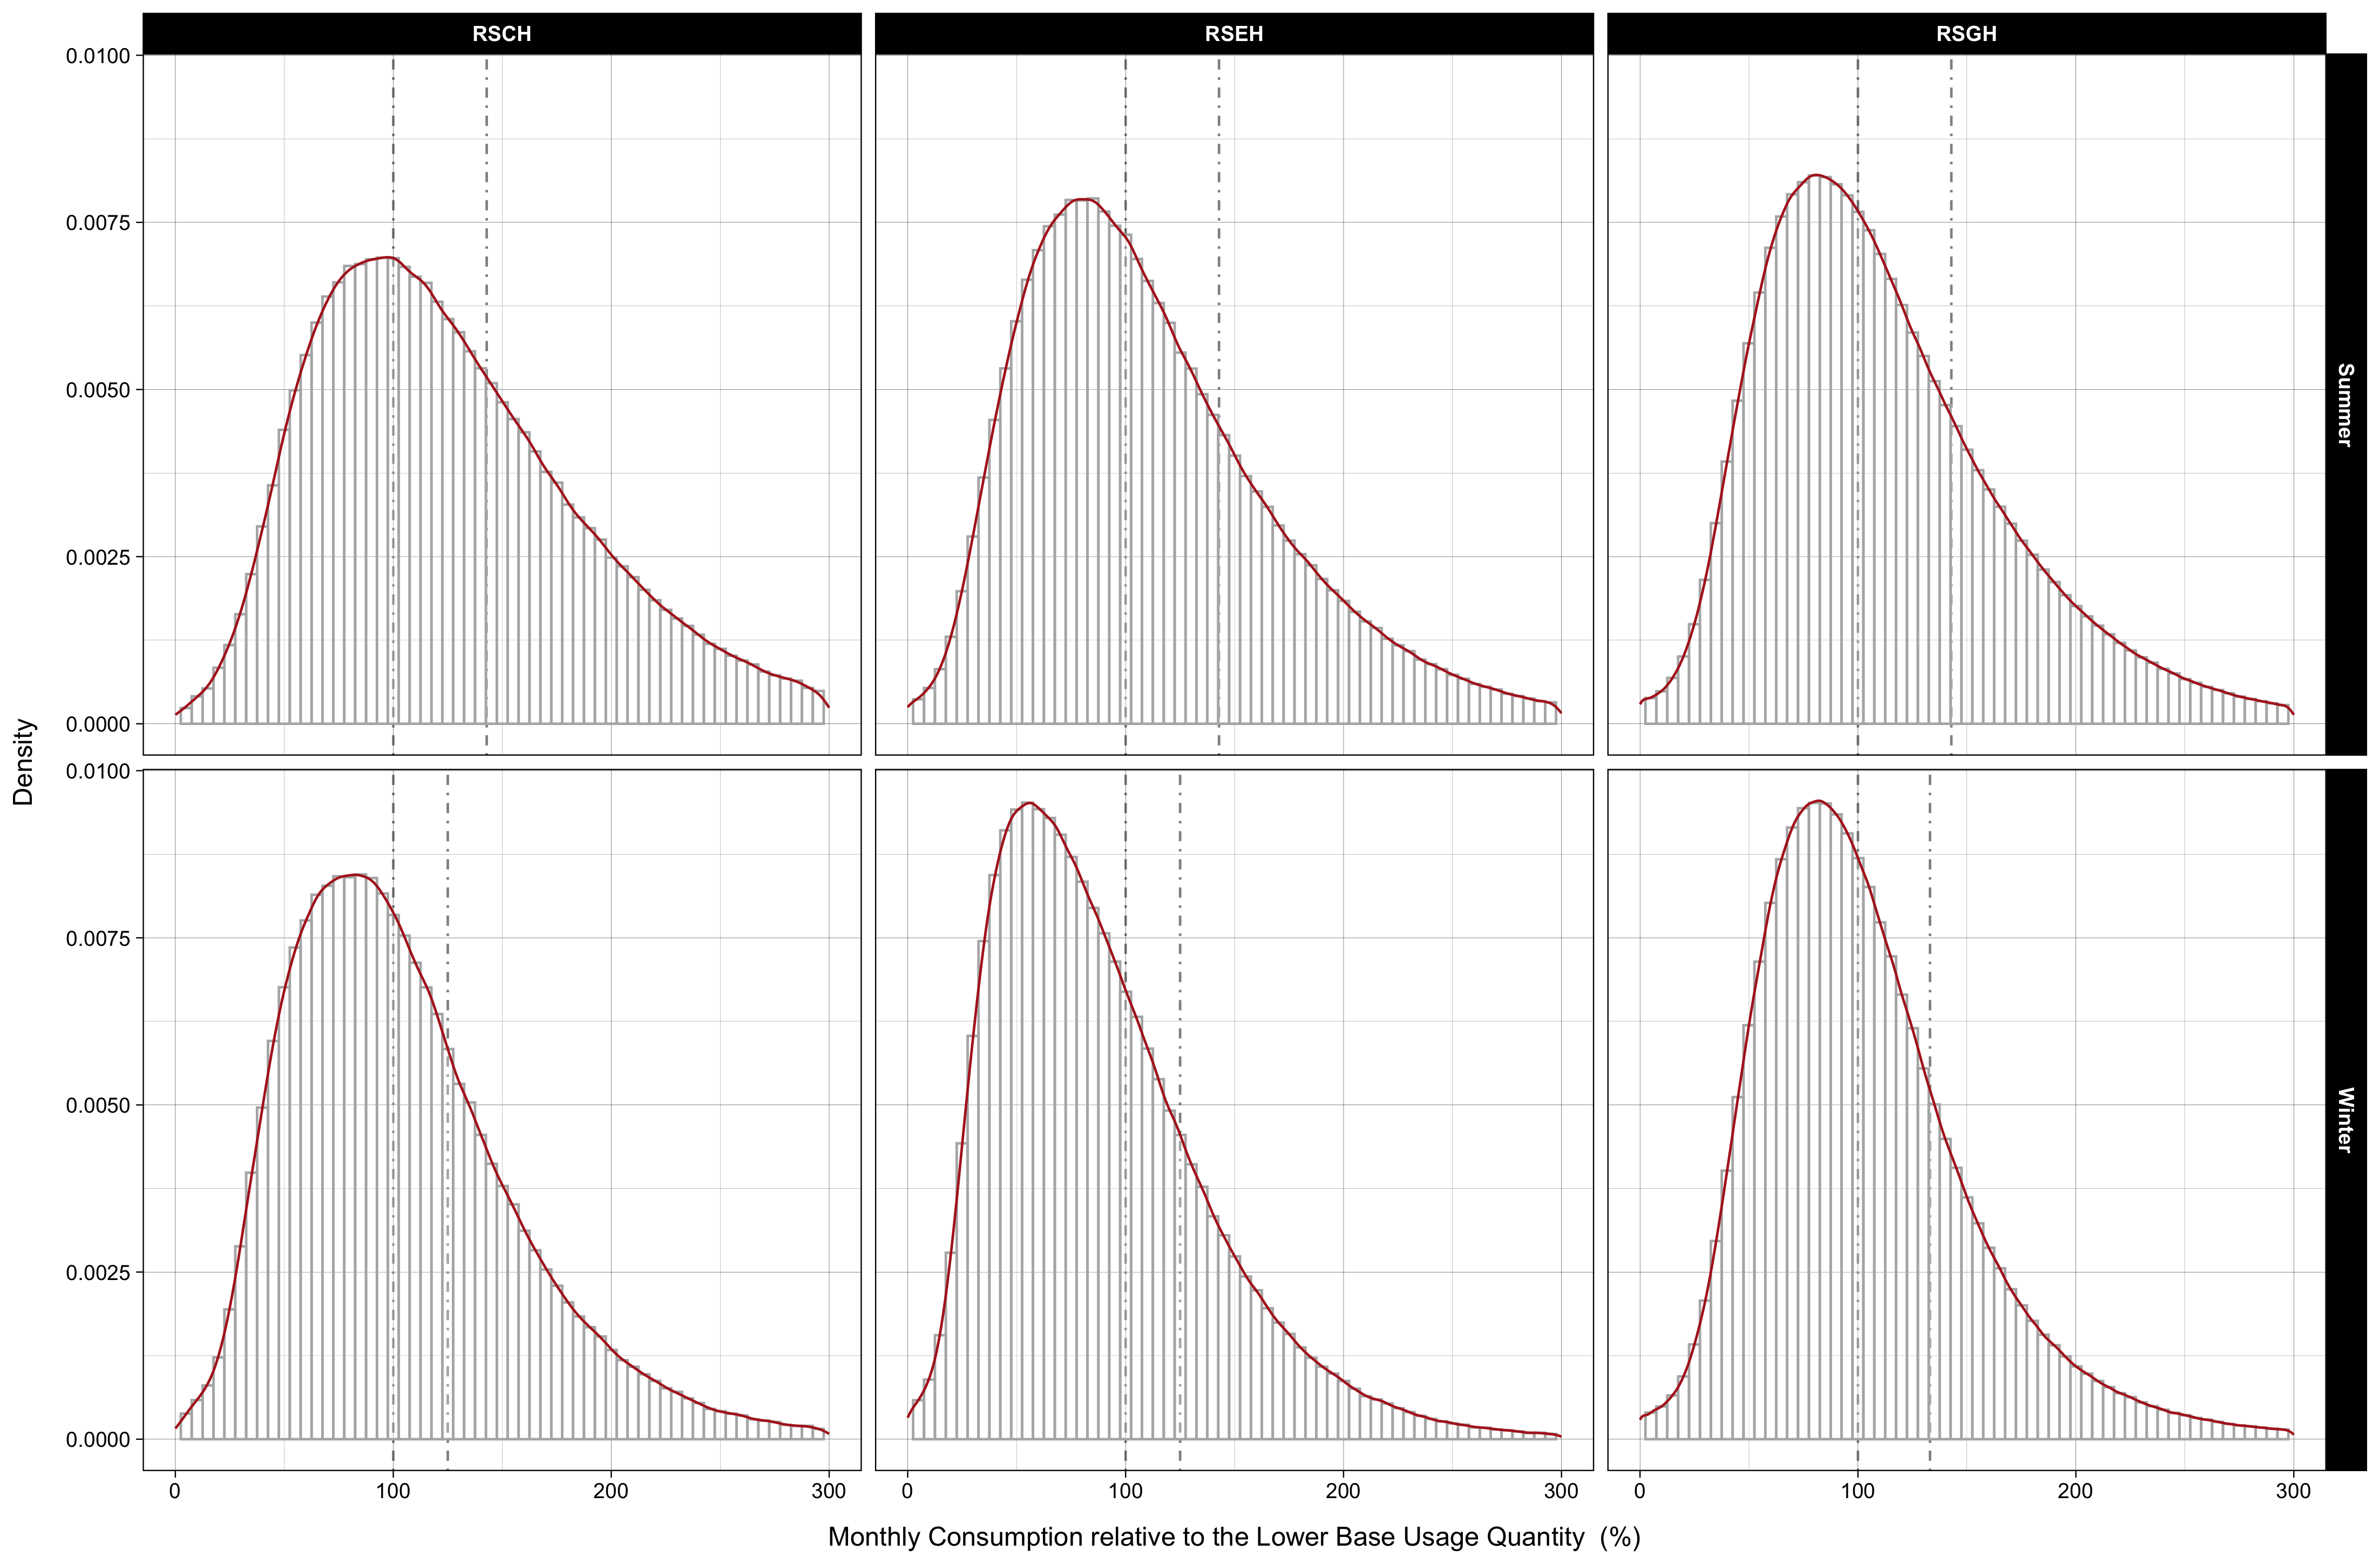
\includegraphics[scale = 0.101]{02_Chapter-1/00A_Figures/Figure_Distribution-of-Electricity-Consumption.png}
        \caption{Distribution of Electricity Consumption by SMUD Residential Customers}
        \caption*{
            {\small
            \textit{Note}: 
            This figure presents histograms, with kernel density estimates, for electricity consumption by SMUD residential customers. Each of the six panels in the figure is for a pair of three major residential rates (i.e., RSCH, RSEH, and RSGH) and two seasons (i.e., summer and winter). Dot-dashed vertical lines in each panel are base usage quantities for the corresponding rate code and season.
        }}
        \label{Figure:SMUD-Billing-Data_Histogram_By-Season-and-Rate-Code}
    \end{figure}
}
Two pieces of evidence support the assumption that base usage quantities do not correspond to jumps in household characteristics. First, as illustrated in Figure \ref{Figure:SMUD-Billing-Data_Histogram_By-Season-and-Rate-Code}, each density plot of the running variable is very smooth, without any bump (i.e., excess mass), around base usage quantities at which marginal prices jump. The set of density plots that show apparent continuity at the thresholds suggests households' inability to precisely adjust their electricity consumption in order not to be subject to a higher marginal price. 

\afterpage{
    \begin{figure}[t!]
        \centering
        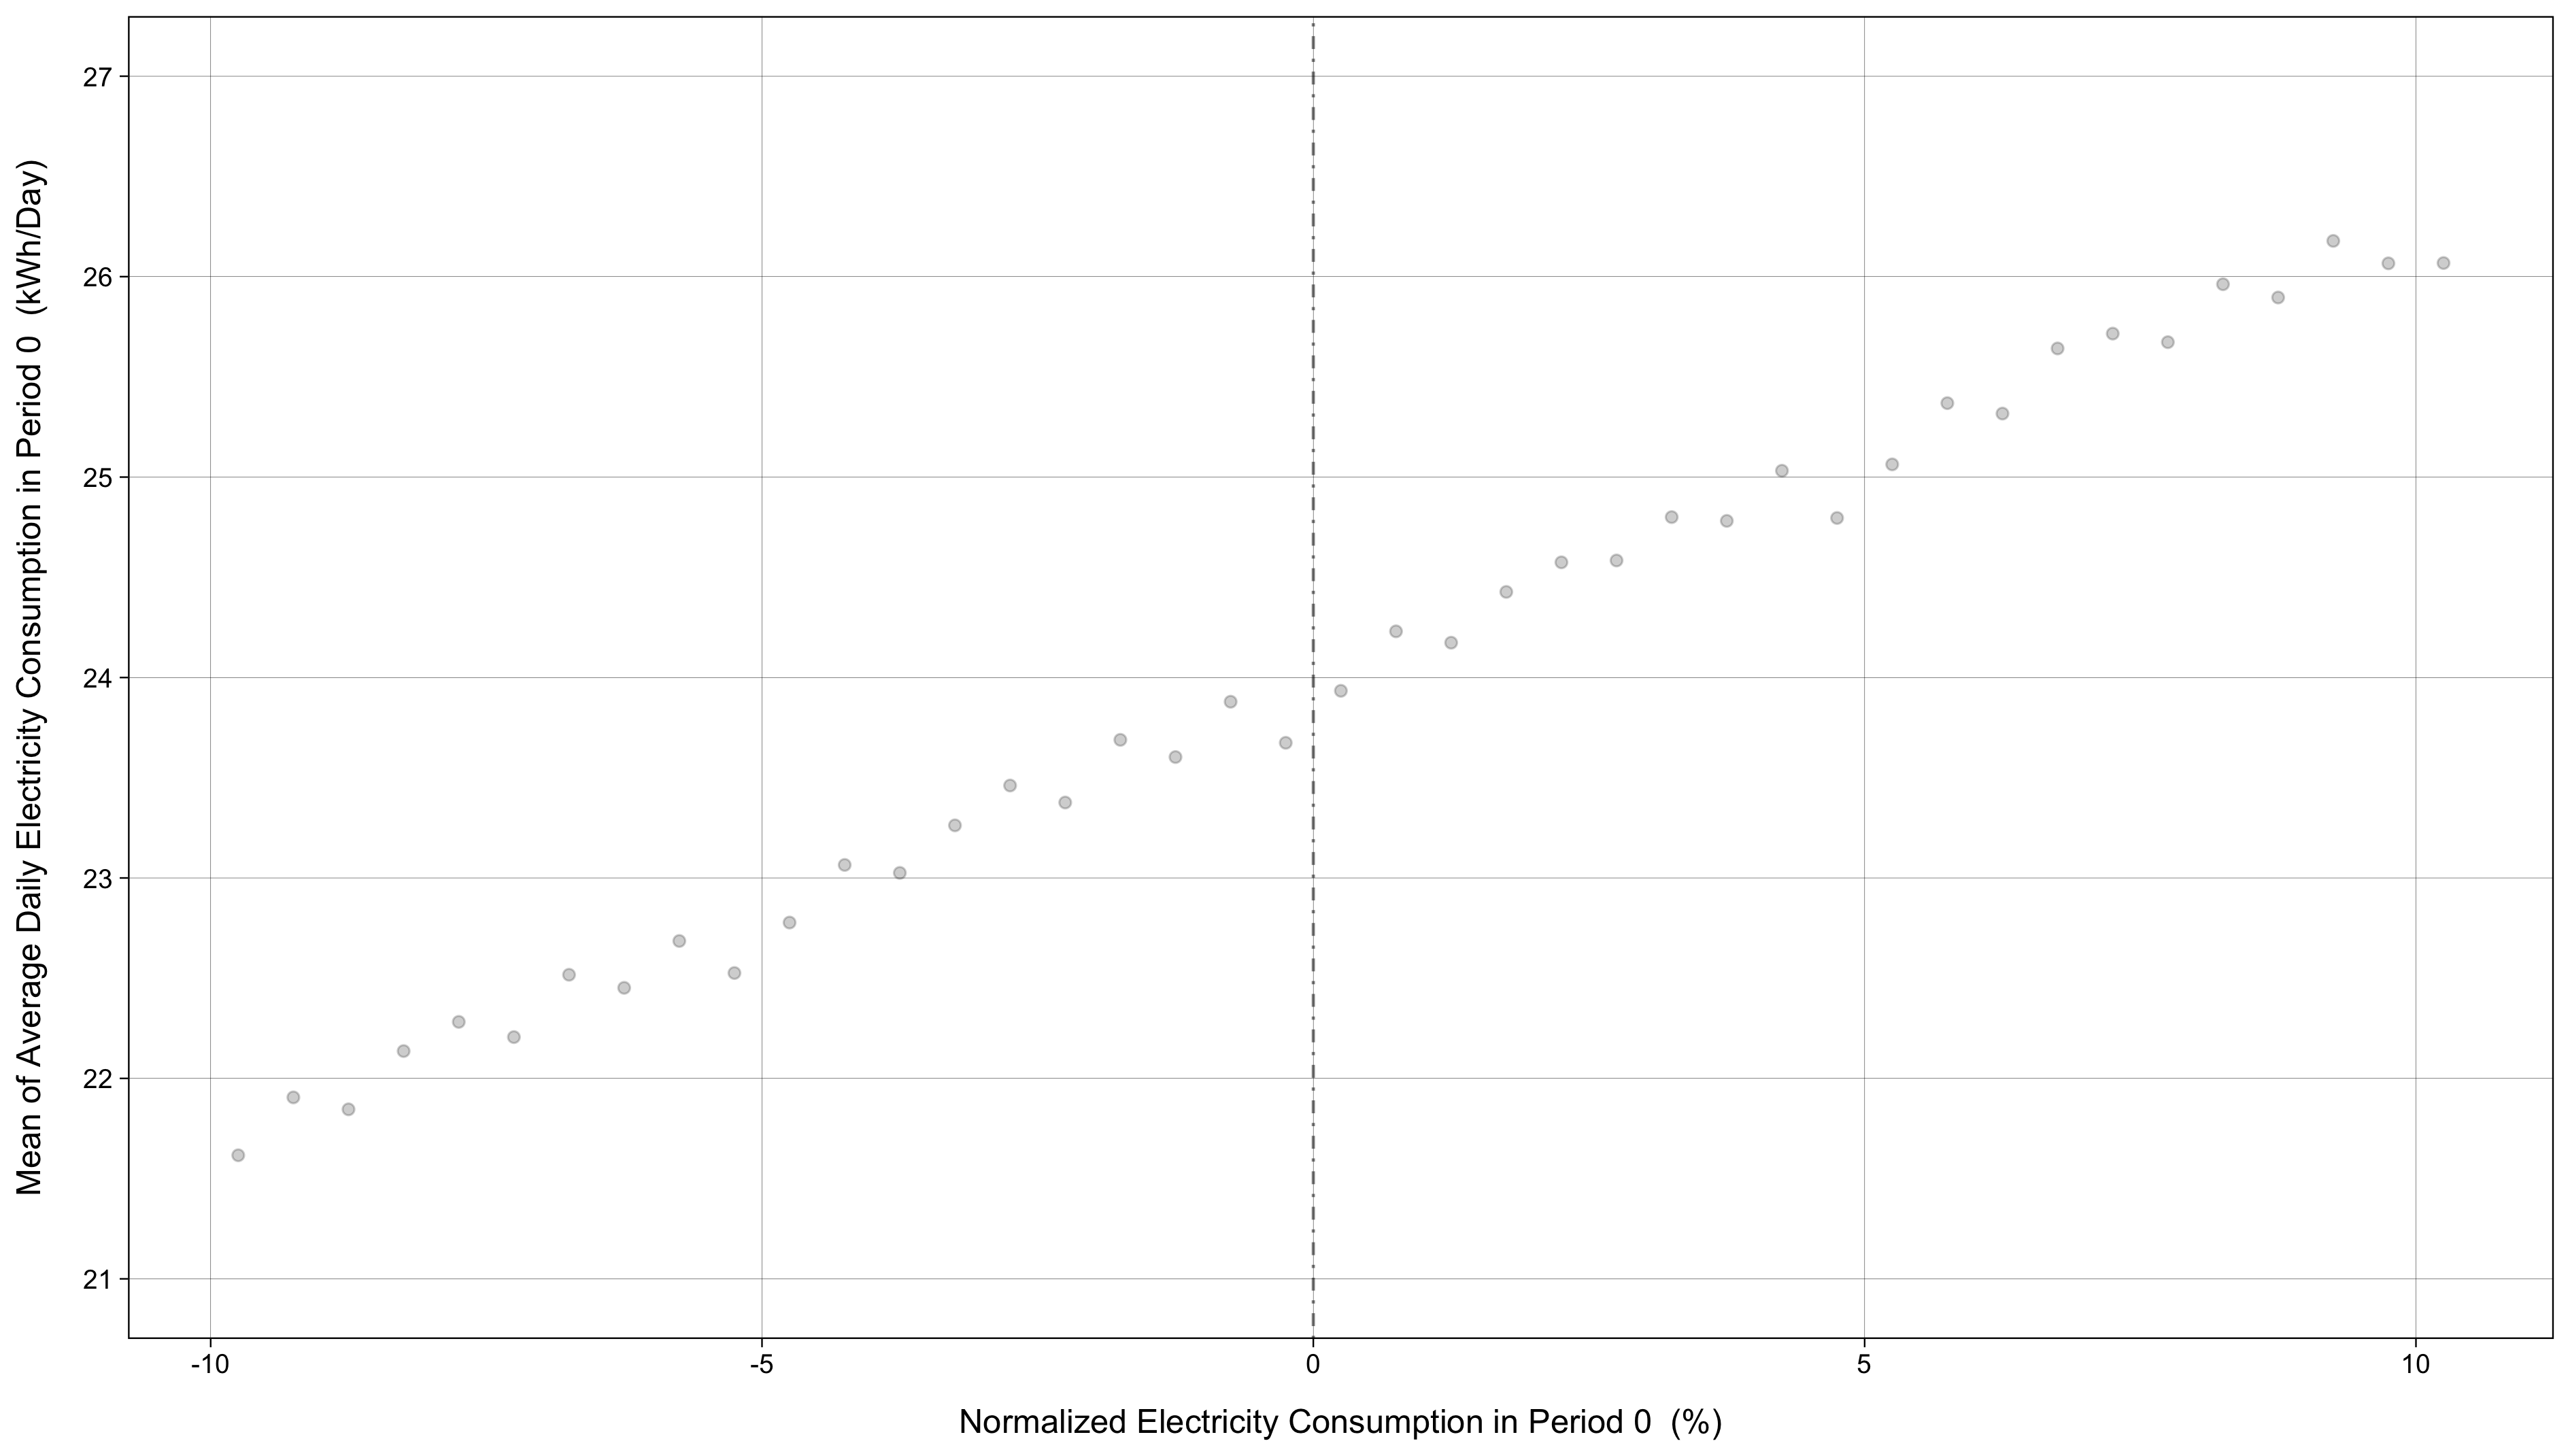
\includegraphics[scale = 0.115]{02_Chapter-1/00A_Figures/Figure_Average-Daily-Electricity-Consumption-in-Period-0-over-NC0.png}
        \caption{Mean of Average Daily Electricity Consumption in Period 0 over $\overline{NC}_{0}$}
        \caption*{
            {\small
            \textit{Note}: 
            In this figure, the scatter points correspond to the average daily electricity consumption in Period 0, calculated by binds with a bandwidth of 1\% of $\overline{NC}_{0}$. As can be seen, the average daily electricity consumption evolves smoothly around the cutoff point (i.e., $\overline{NC}_{0} = 0$). 
        }}
        \label{Figure:Average-Daily-Electricity-Consumption-in-Period-0-over-NC0}
    \end{figure}
}
Second, Figure \ref{Figure:Average-Daily-Electricity-Consumption-in-Period-0-over-NC0} demonstrates that households' average daily electricity consumption during Period 0 evolved smoothly around the lower cutoff point. This figure allows me, at a minimum, not to reject the assumption of local randomization around the base usage quantity, even though examining an observed covariate around the thresholds is not also a direct test for the validity of the assumption.

